\section{Validation: Epoch-Budget Sensitivity and Implementation Audit}
\label{sec:phase4}

Every result in Sections~\ref{sec:phase1}--\ref{sec:track-e} was measured at
a fixed $10^4$-epoch budget, a tenth of the base paper's, for the cost reasons
of Section~\ref{sec:budget}. This stage asks whether that budget is long
enough for the \emph{rankings} to be trusted, and whether any gap to the
paper is due to the budget or to an implementation difference.

\begin{expectbox}
\expectrow{Question}{Do the conclusions drawn at $10^4$ epochs survive five times the training budget?}
\expectrow{Expected}{Absolute errors fall; orderings between configurations hold, since every $10^4$-epoch model had already reached a training loss near $10^{-4}$.}
\expectrow{Observed}{Three of four conclusions hold. The fourth, the one the paper headlines, reverses: at $5\times10^4$ epochs the parameter-matched MLP extrapolates $6.8\times$ \emph{better} than KAN-ODE.}
\end{expectbox}

\subsection{Design}

Five configurations were chosen to test the specific conclusions most
exposed to the budget: Euler (the one solver short of $10^{-4}$ at $10^4$
epochs), Tsit5/RBF (the reference), B-spline (the near-tie with RBF), and both
MLP baselines. Each was retrained from scratch at $5\times10^4$ epochs with the
recipe of Table~\ref{tab:recipe} unchanged, on cloud CPUs. The B-spline run
was cut to $2.5\times10^4$ epochs because its short calibration run
predicted about 35 hours for the full budget; the real run turned out
$1.63\times$ faster than that calibration ($1.544$ against $2.52$~s/epoch),
a reminder that a five-epoch sample is dominated by start-up cost. The batch
used $23.2$ serial CPU-hours against a planned $17.0$, and $10.7$ hours of
wall-clock with the five jobs in parallel. Before analysis every
\path{metrics.json} was checked against its \path{training_history.json}
epoch count, and every checkpoint was reloaded and re-scored; the rollouts
reproduce the stored extrapolation MSE to within $0.6\%$.

\subsection{Results}

\begin{table}[!ht]
\centering
\footnotesize
\renewcommand{\arraystretch}{1.1}
\caption{The five configurations at $10^4$ epochs (Section~\ref{sec:phase2})
and at the extended budget. ``Clip'' is the fraction of optimizer steps on
which gradient clipping at norm $1.0$ engaged; $\|\nabla\|_{\text{med}}$ is
the median pre-clip gradient norm over the extended run.}
\label{tab:phase4}
\begin{tabular}{@{}L{2.6cm} C{0.9cm} C{1.7cm} C{1.7cm} C{1.35cm} C{0.8cm} C{1.0cm} C{1.3cm}@{}}
\toprule
\hdrrow \thh{Configuration} & \thh{Epochs} & \thh{Training MSE} & \thh{Extrap.\ MSE} & \thh{Extrap.\ $R^2$} & \thh{$\hat L$} & \thh{Clip} & \thh{$\|\nabla\|_{\text{med}}$}\\
\midrule
Euler / RBF & 10k & $1.38\times10^{-4}$ & $2.51\times10^{-3}$ & $0.99914$ & $8.55$ & & \\
 & \textbf{50k} & $8.85\times10^{-6}$ & $1.93\times10^{-4}$ & $0.99993$ & $7.72$ & $4.7\%$ & $0.147$\\
\addlinespace
Tsit5 / RBF & 10k & $8.83\times10^{-5}$ & $8.92\times10^{-5}$ & $0.99997$ & $6.91$ & & \\
 & \textbf{50k} & $6.59\times10^{-6}$ & $4.02\times10^{-5}$ & $0.999986$ & $7.75$ & $4.3\%$ & $0.169$\\
\addlinespace
Tsit5 / B-spline & 10k & $7.20\times10^{-5}$ & $8.38\times10^{-5}$ & $0.99997$ & $8.44$ & & \\
 & \textbf{25k} & $9.65\times10^{-6}$ & $4.26\times10^{-5}$ & $0.999985$ & $7.05$ & $2.2\%$ & $0.033$\\
\addlinespace
MLP-ODE, SiLU & 10k & $9.50\times10^{-5}$ & $4.77\times10^{-4}$ & $0.99984$ & $5.07$ & & \\
 & \textbf{50k} & $\mathbf{1.82\times10^{-6}}$ & $\mathbf{5.90\times10^{-6}}$ & $\mathbf{0.999998}$ & $5.65$ & $11.1\%$ & $0.162$\\
\addlinespace
MLP-ODE, tanh (paper) & 10k & $1.08\times10^{0}$ & $1.69\times10^{0}$ & $0.4215$ & $38.2$ & & \\
 & \textbf{50k} & $1.01\times10^{0}$ & $4.32\times10^{0}$ & $-0.4841$ & $104.8$ & $99.3\%$ & $19.8$\\
\bottomrule
\end{tabular}
\end{table}

\begin{figure}[htbp]
\centering
\begin{subfigure}[b]{0.49\textwidth}
  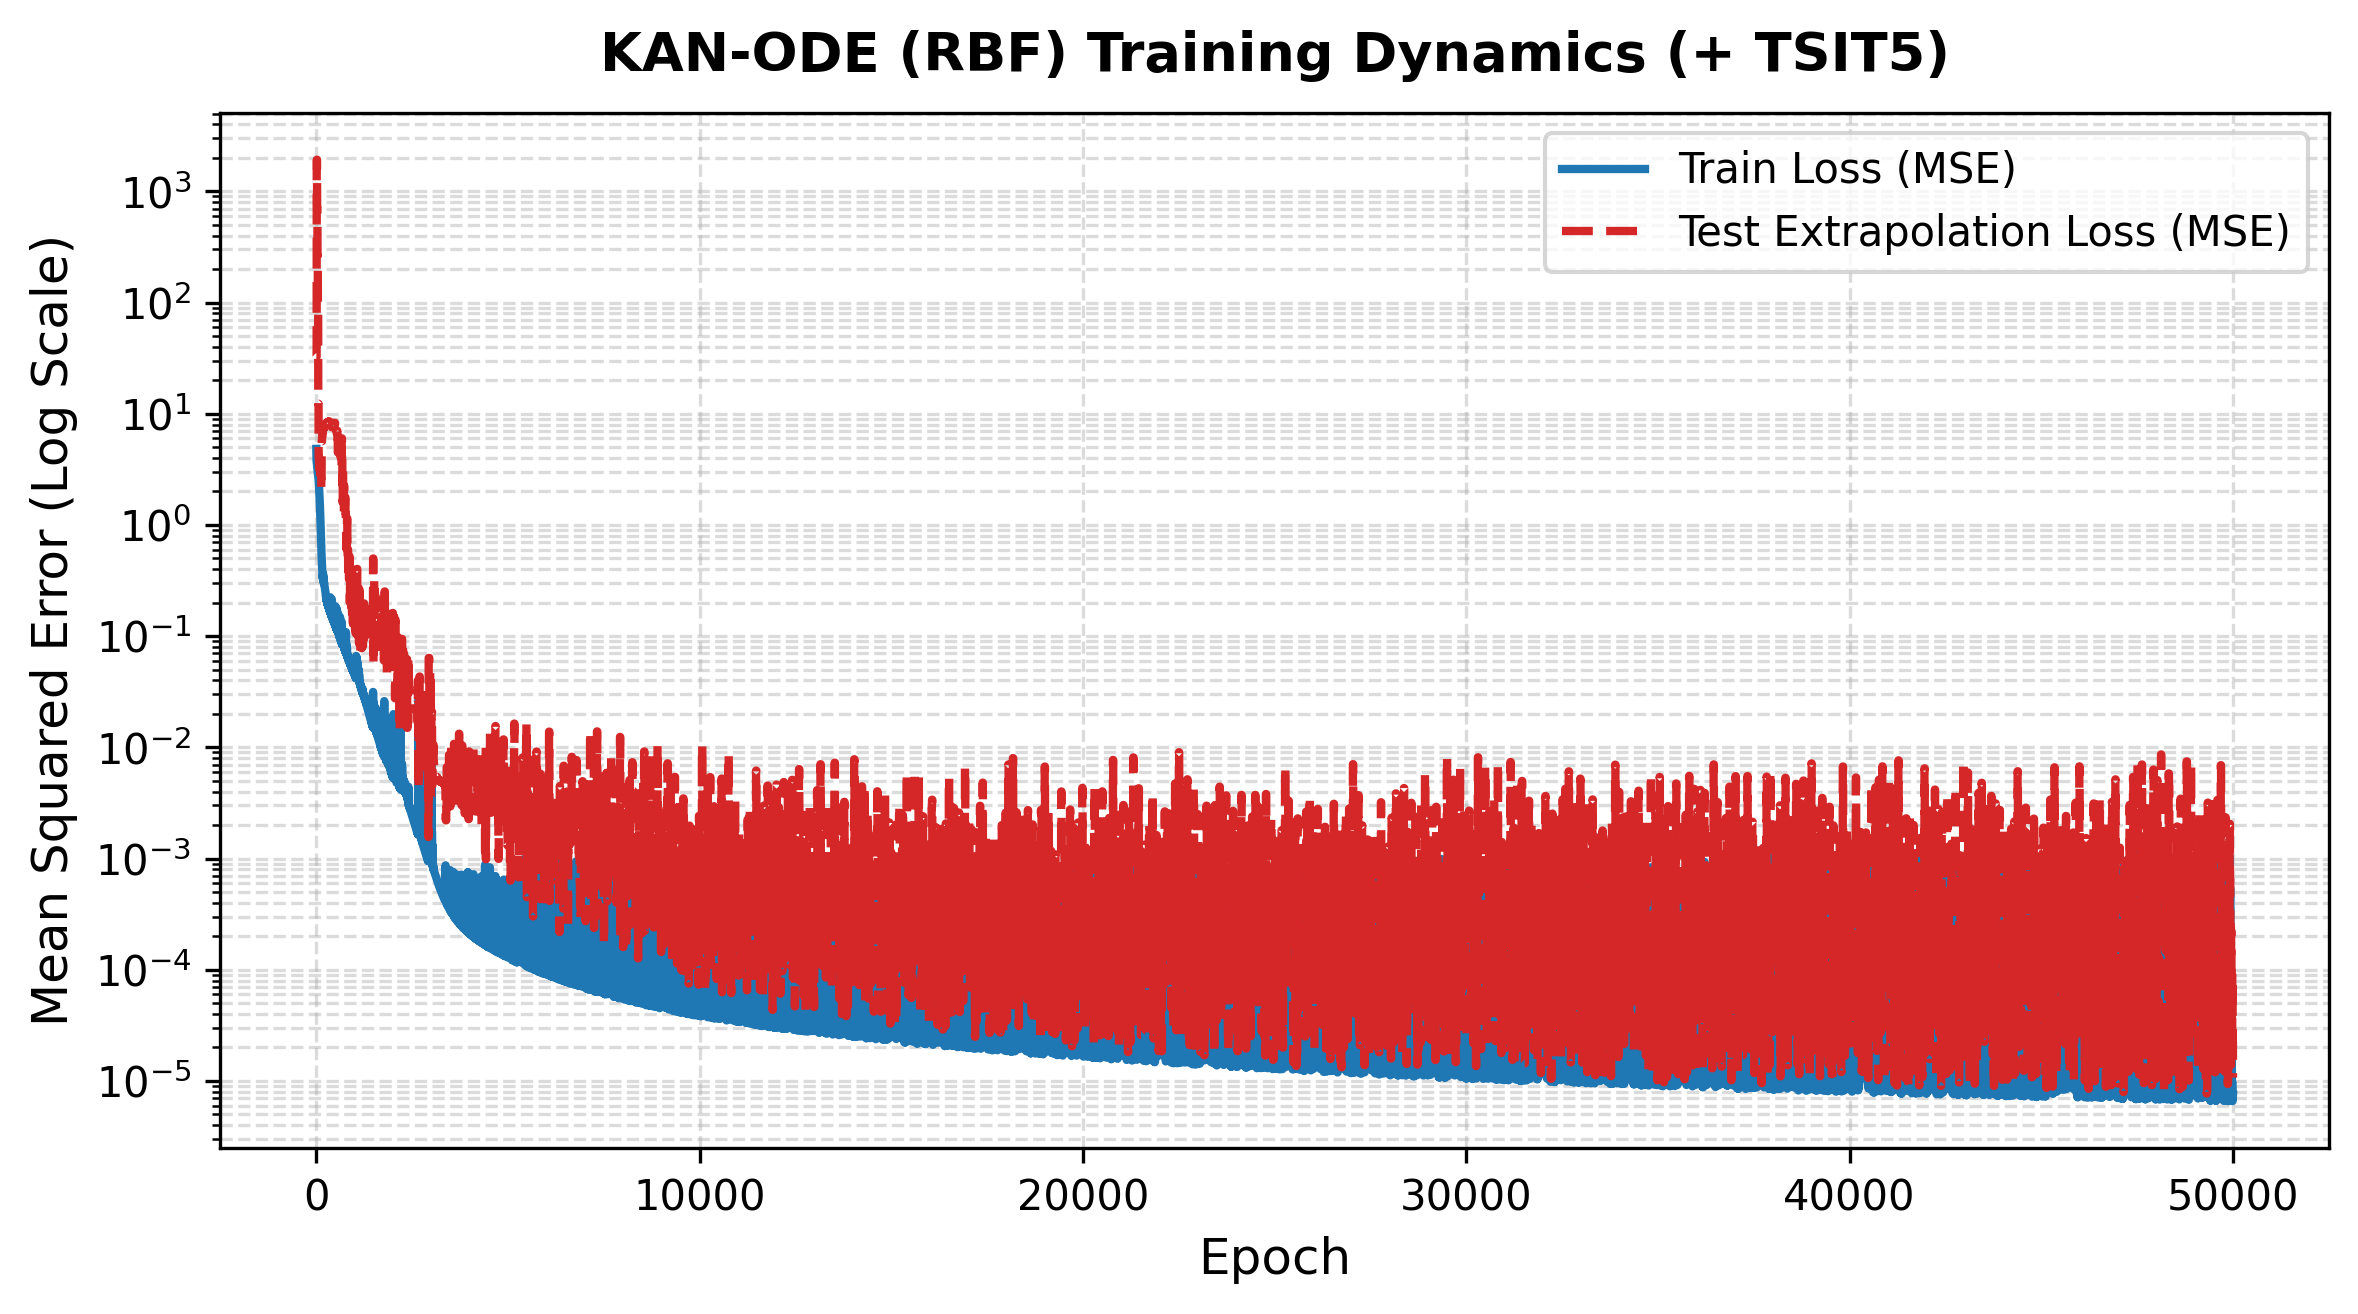
\includegraphics[width=\linewidth]{figures/phase4/tsit5_rbf_50k_loss_curves.png}
  \caption{KAN-ODE, Tsit5 / RBF, 50k}
\end{subfigure}\hfill
\begin{subfigure}[b]{0.49\textwidth}
  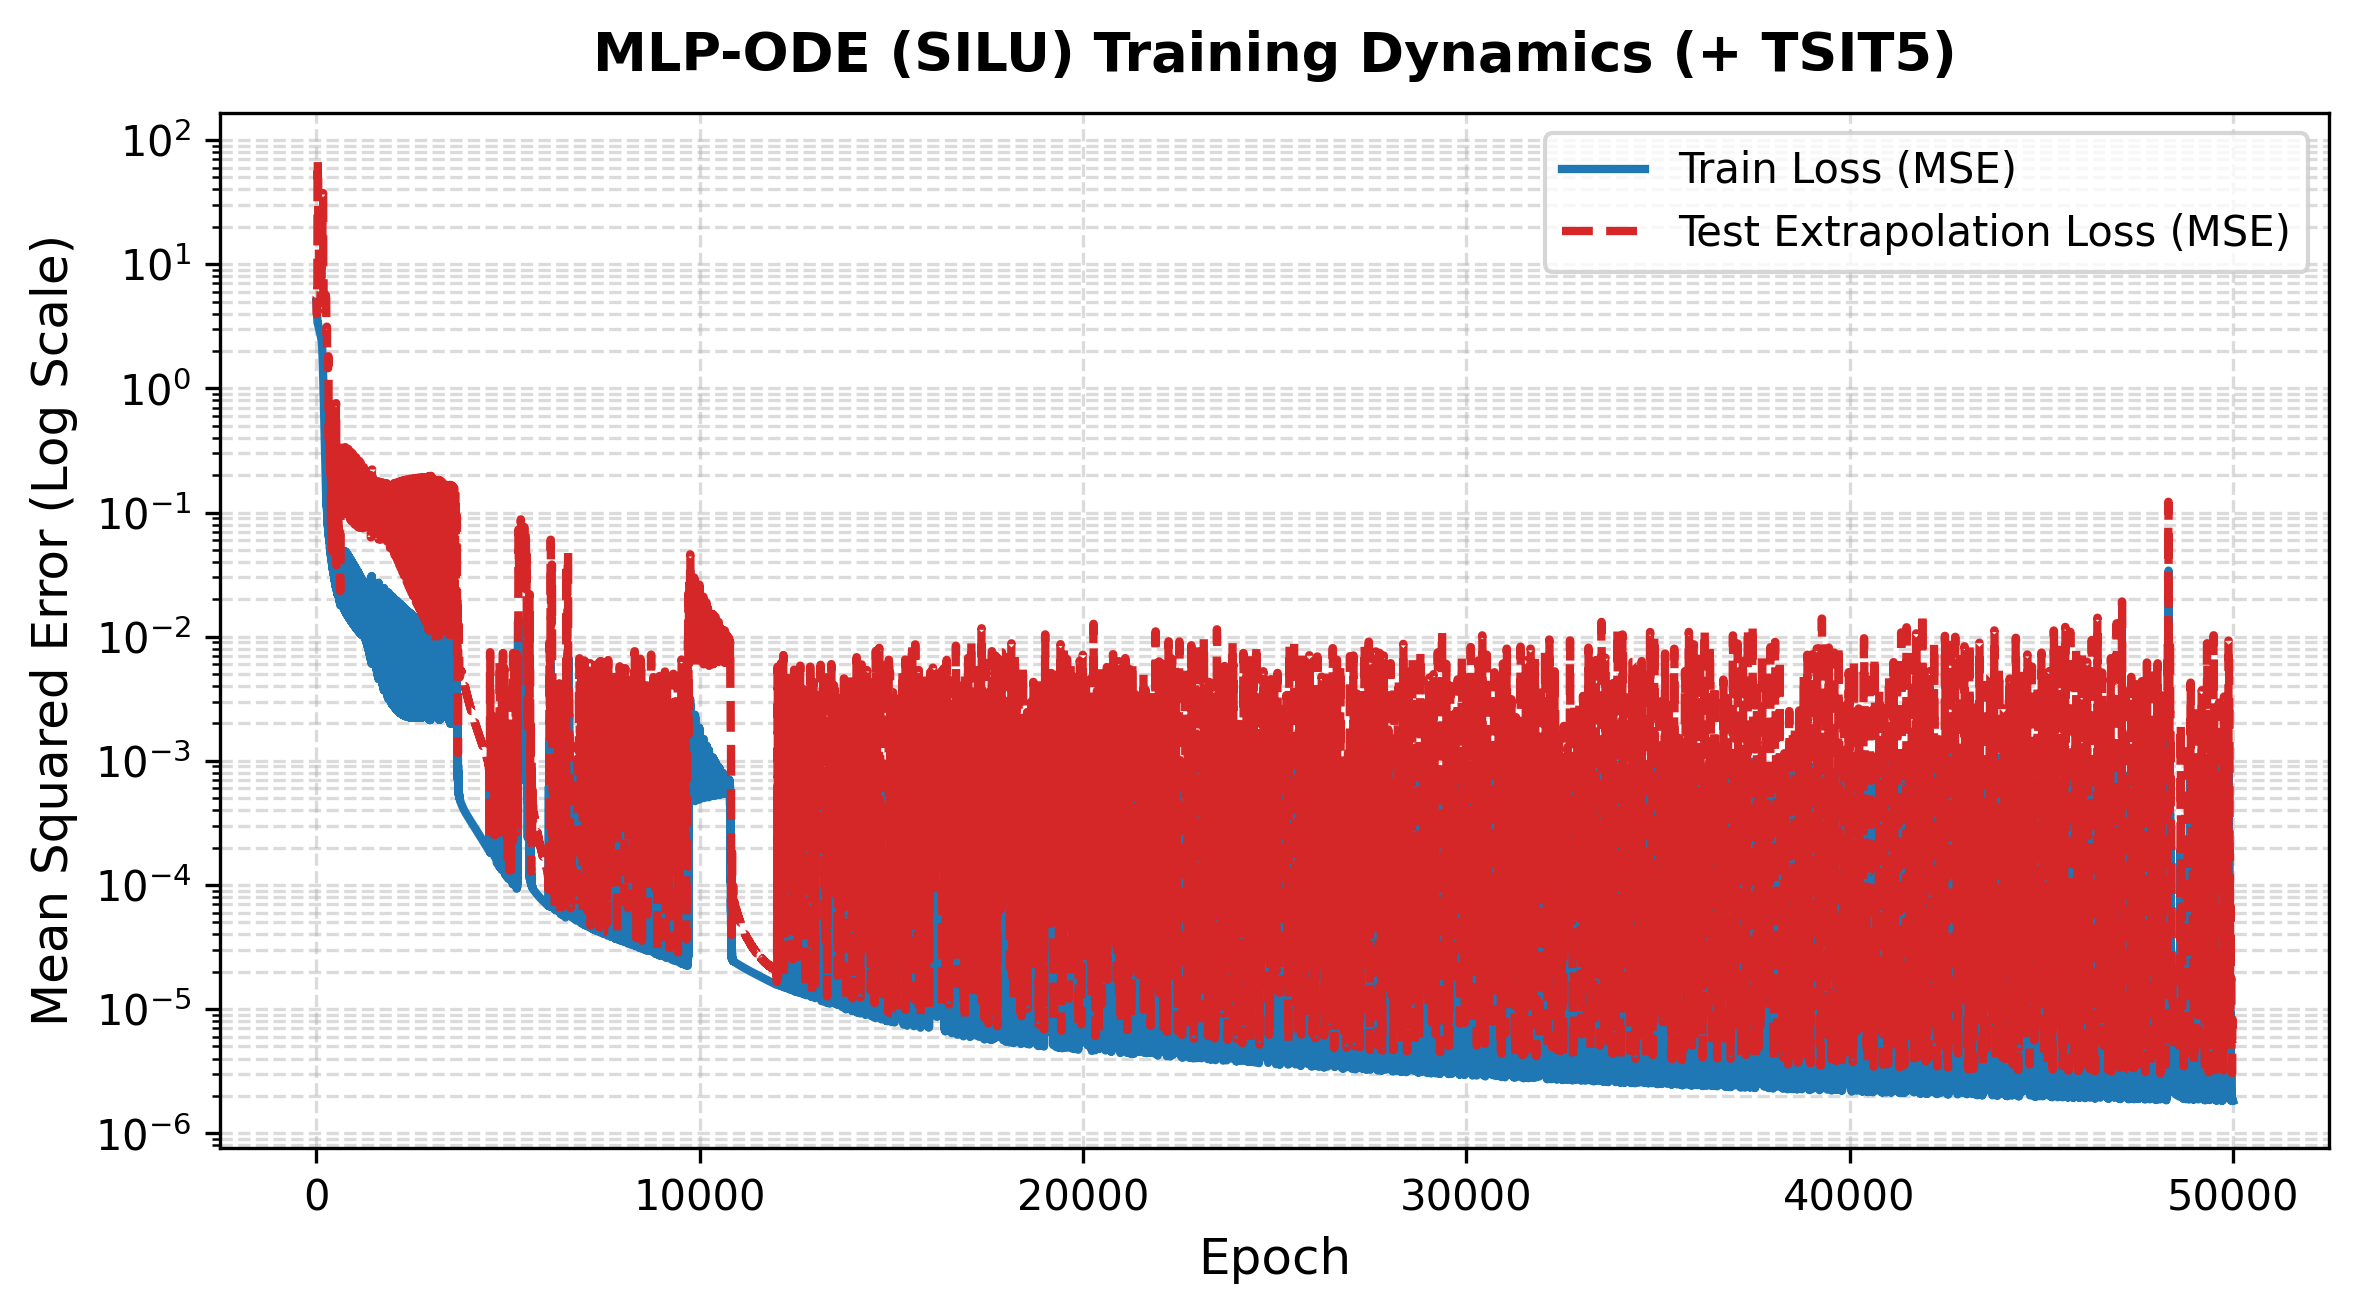
\includegraphics[width=\linewidth]{figures/phase4/mlp_silu_50k_loss_curves.png}
  \caption{MLP-ODE, SiLU, 50k}
\end{subfigure}\\[4pt]
\begin{subfigure}[b]{0.49\textwidth}
  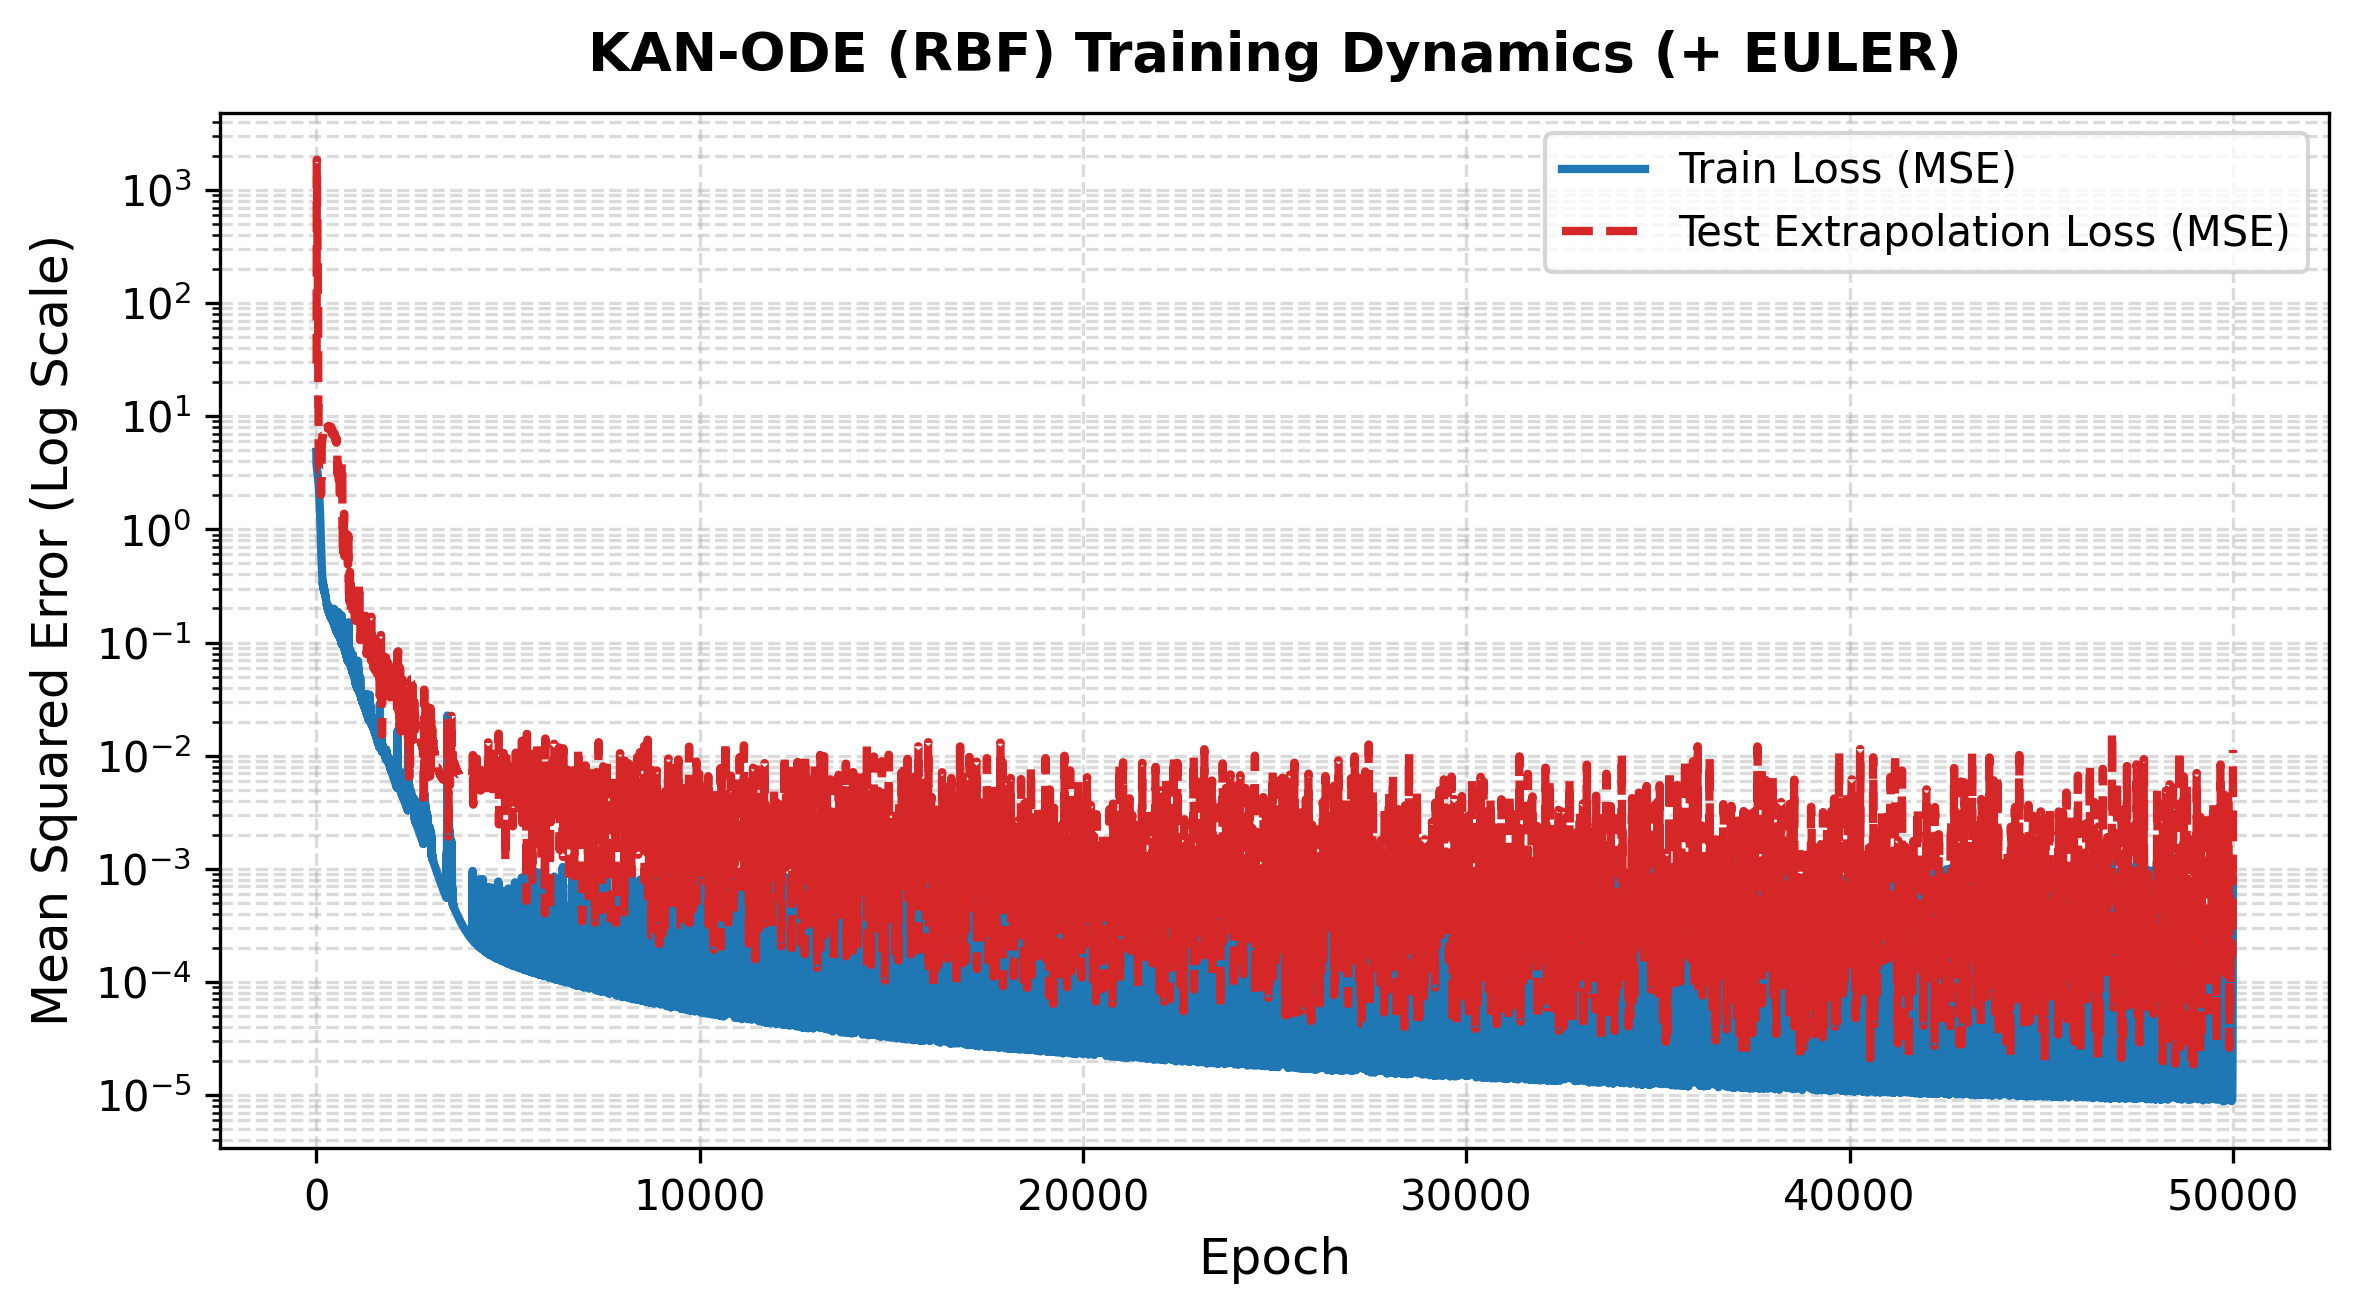
\includegraphics[width=\linewidth]{figures/phase4/euler_50k_loss_curves.png}
  \caption{KAN-ODE, Euler / RBF, 50k}
\end{subfigure}\hfill
\begin{subfigure}[b]{0.49\textwidth}
  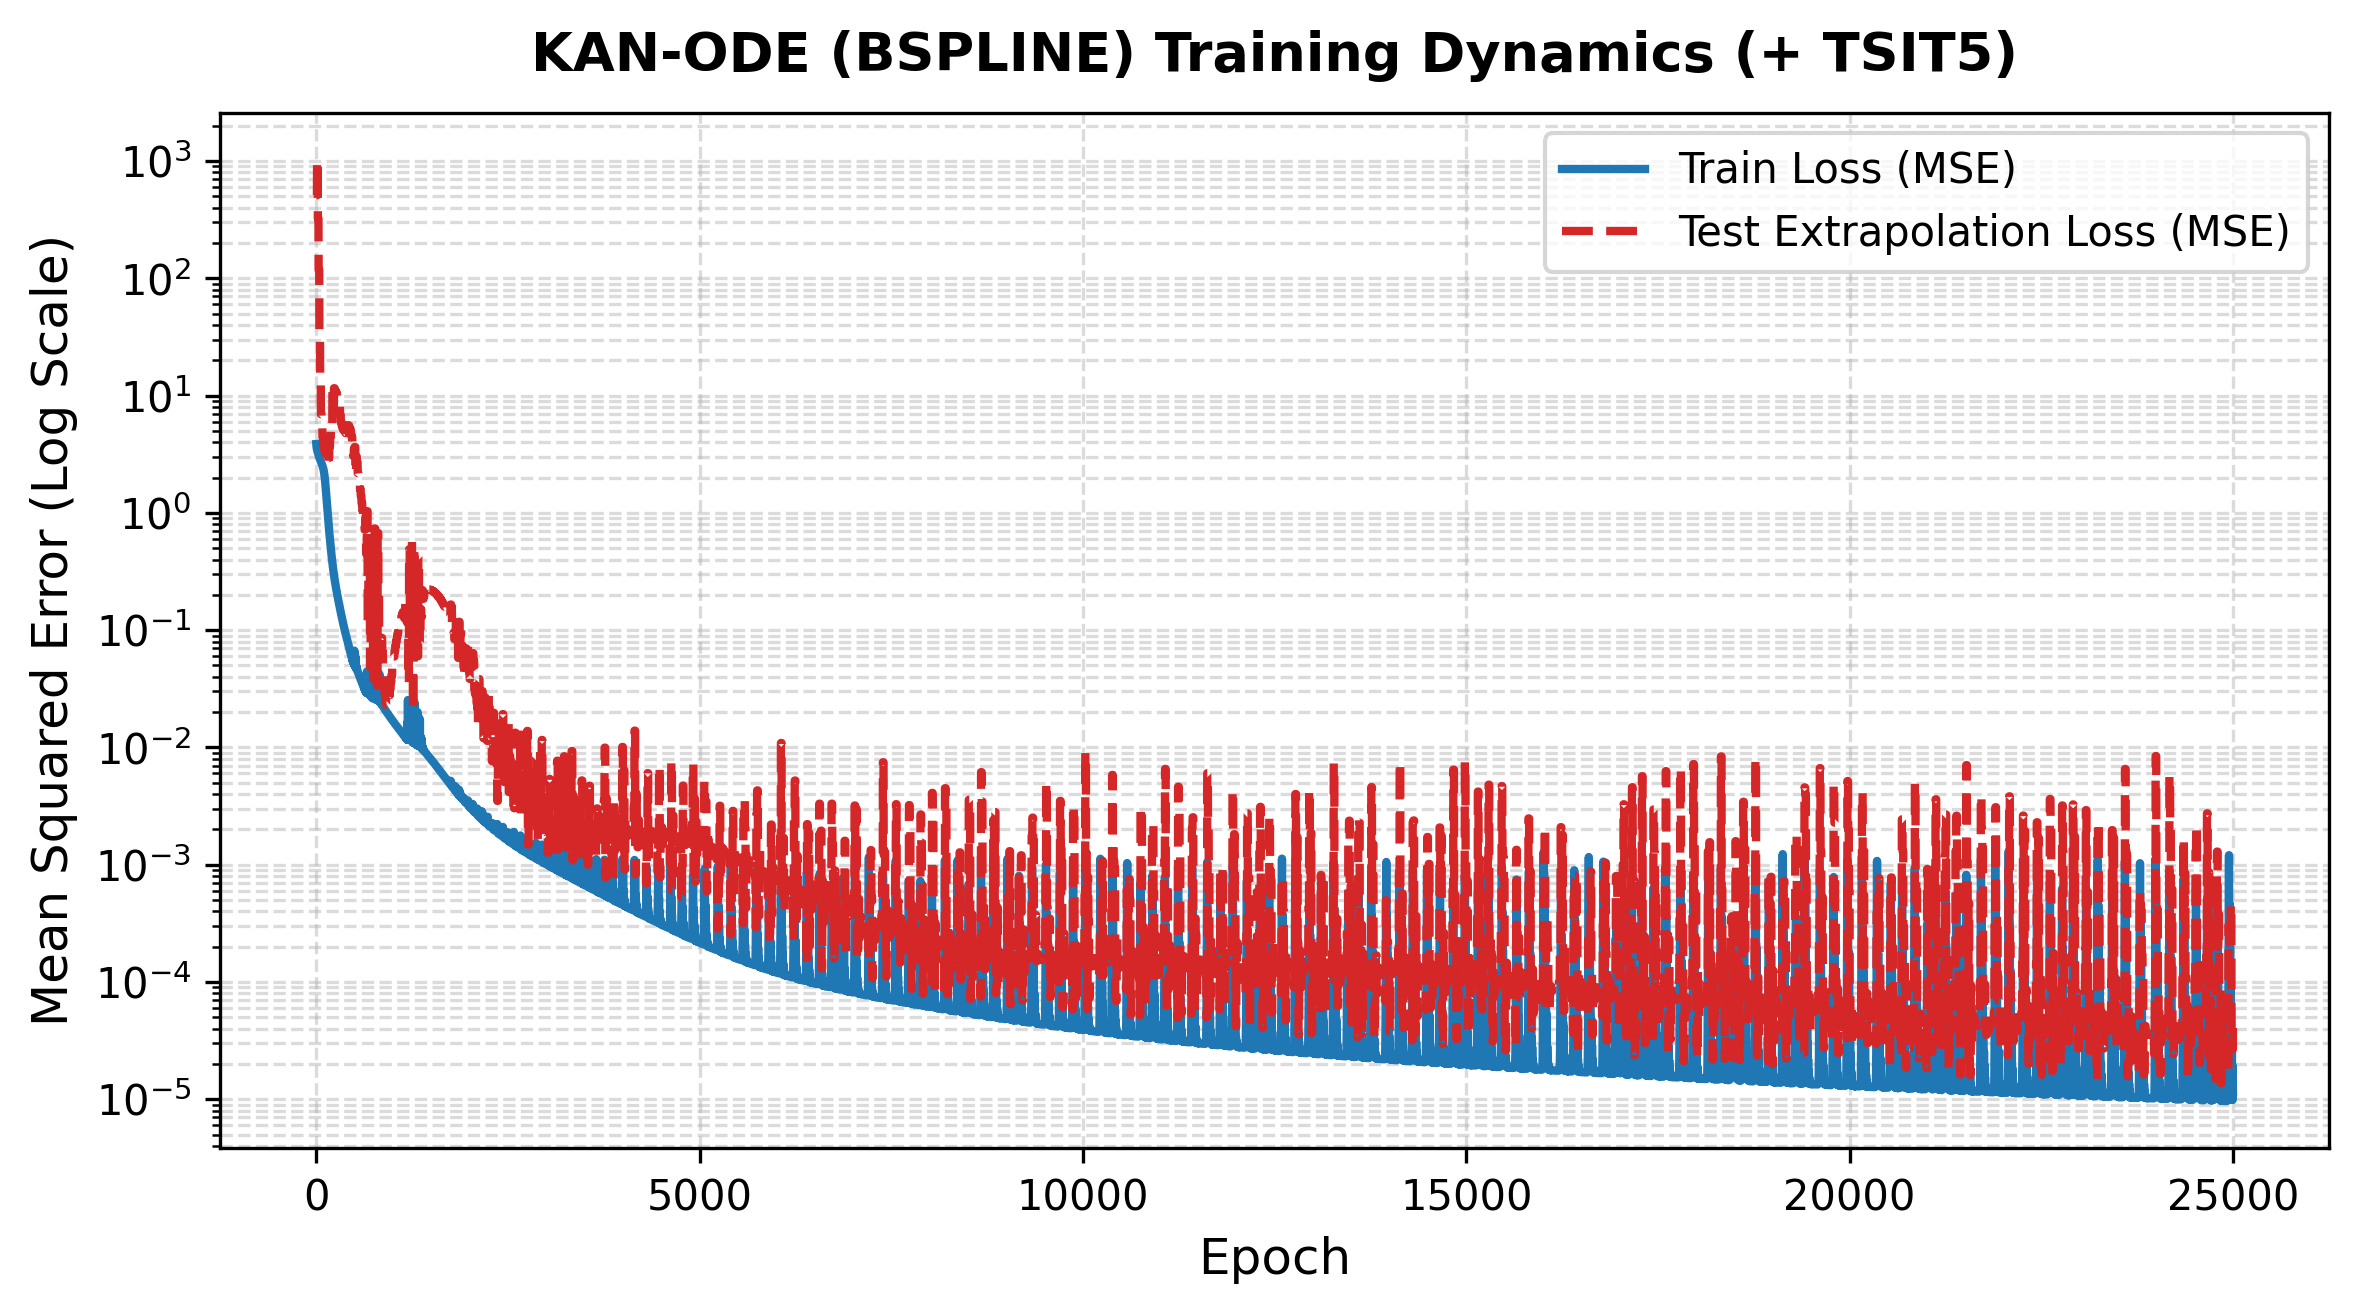
\includegraphics[width=\linewidth]{figures/phase4/bspline_25k_loss_curves.png}
  \caption{KAN-ODE, Tsit5 / B-spline, 25k}
\end{subfigure}\\[4pt]
\begin{subfigure}[b]{0.49\textwidth}
  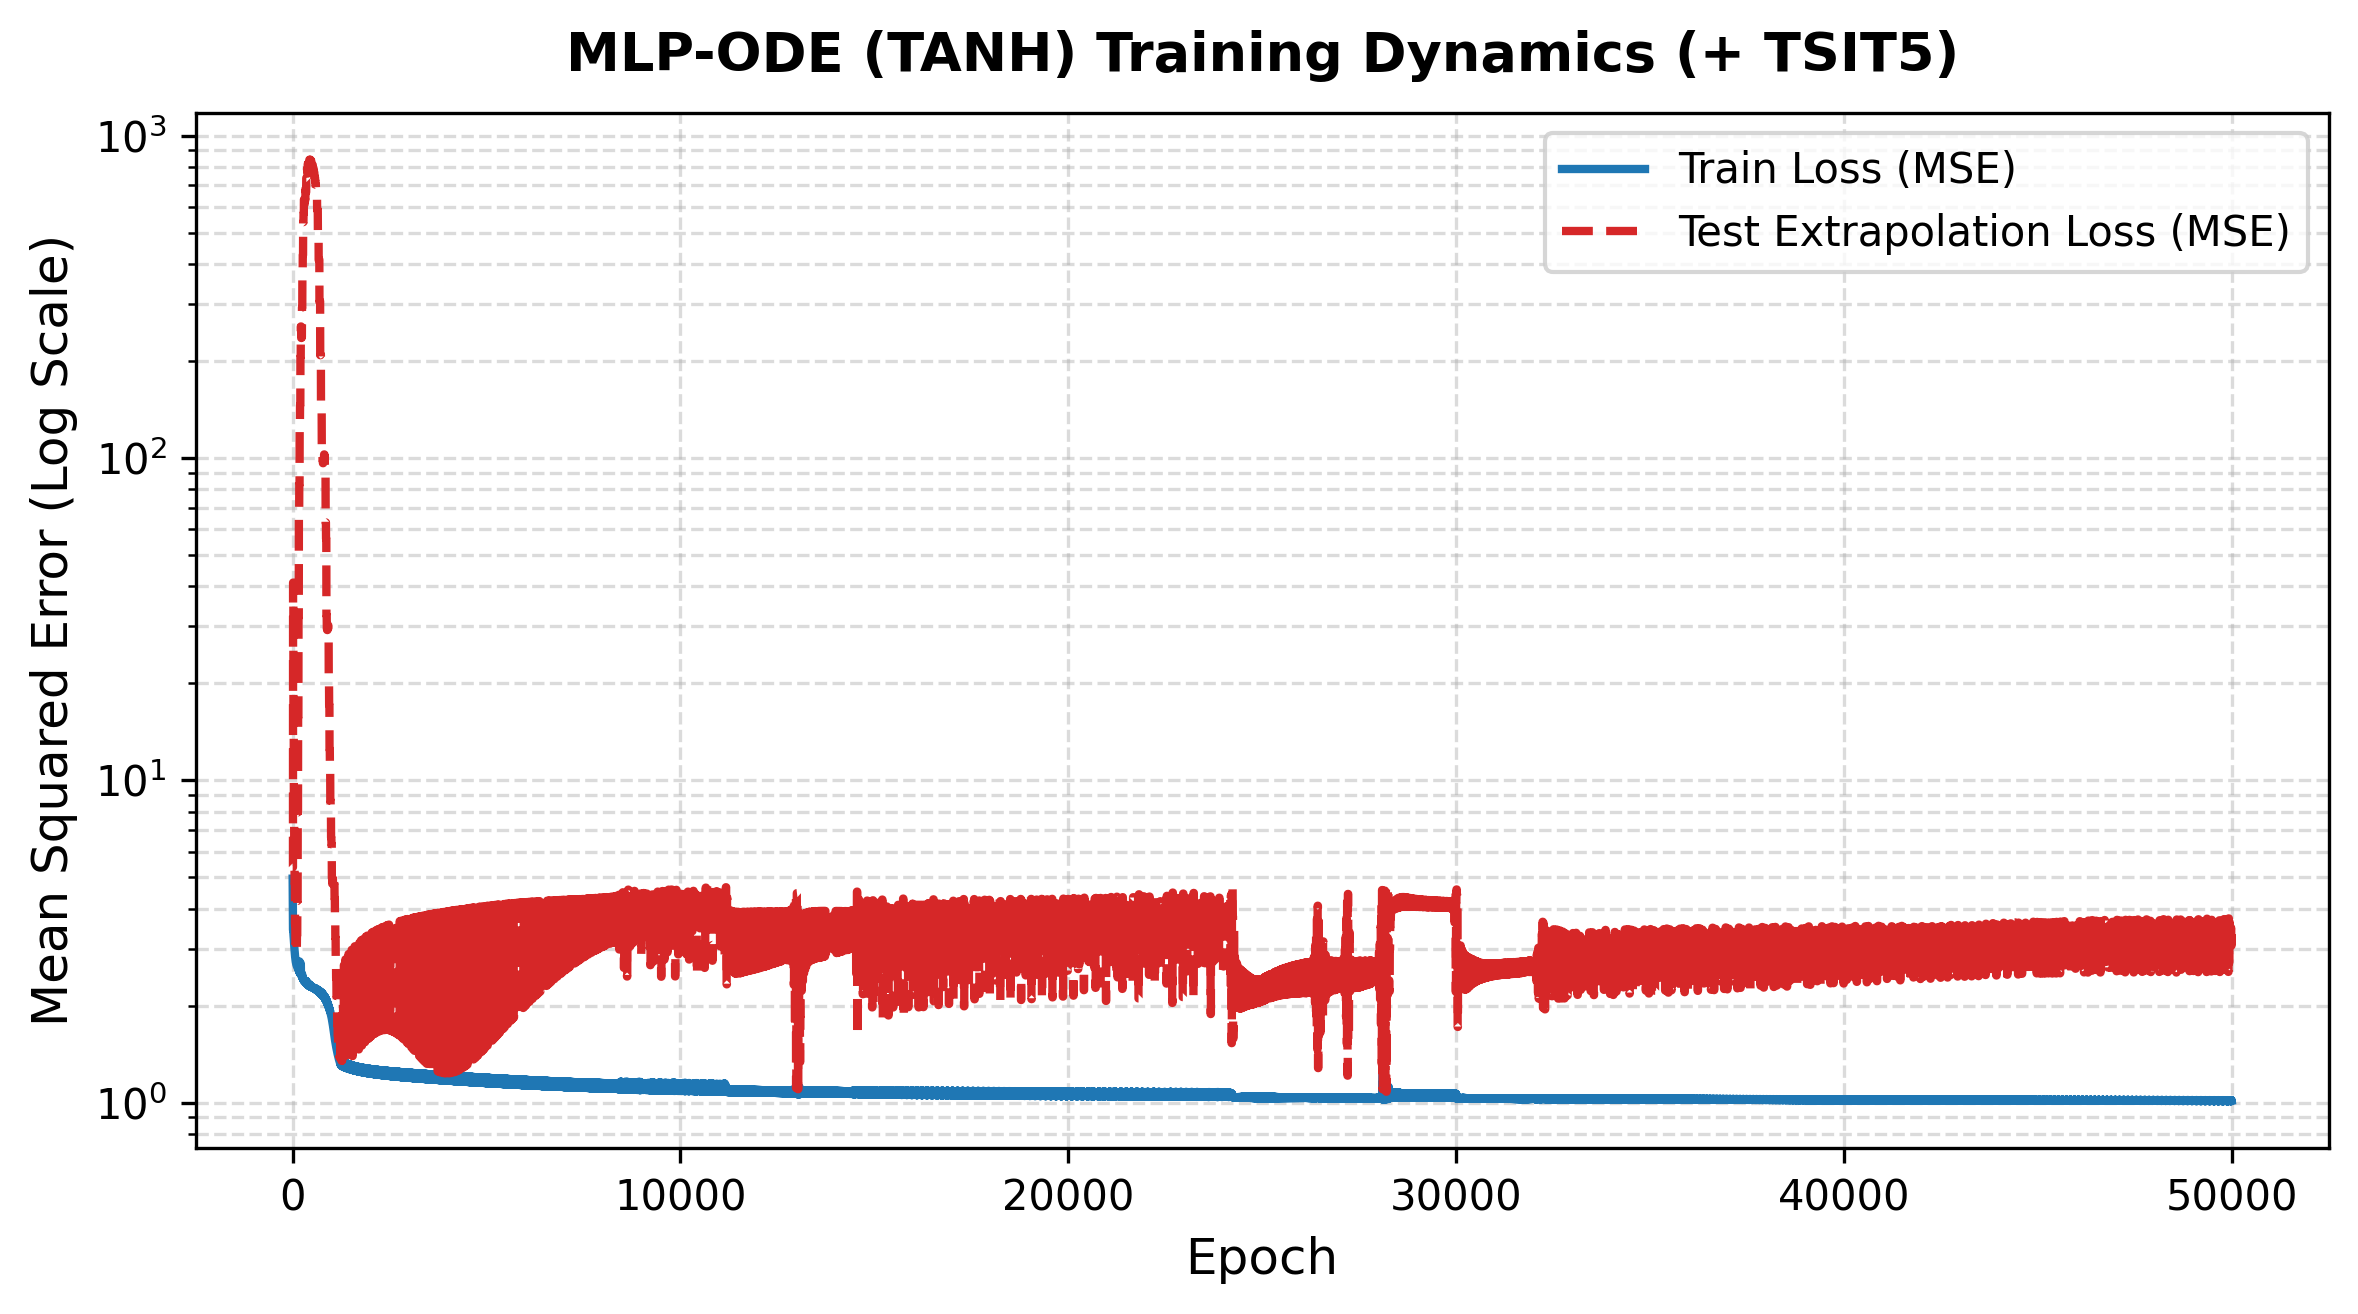
\includegraphics[width=\linewidth]{figures/phase4/mlp_paperspec_50k_loss_curves.png}
  \caption{MLP-ODE, tanh (paper spec), 50k}
\end{subfigure}
\caption{Training and test loss of the five extended runs, as saved by each
run. Training loss is logged every epoch; the test loss (full horizon
$[0,14]$) every ten epochs, and it spikes by up to two orders of magnitude
throughout, which is why the comparison in the text uses a 500-epoch rolling
median rather than raw values.}
\label{fig:phase4-curves}
\end{figure}

Every working configuration improves its training MSE by $7.5$--$52\times$
(Table~\ref{tab:phase4}); what matters is which orderings survive.
Table~\ref{tab:phase4-verdicts} states the verdict for each conclusion the
earlier sections draw.

\begin{table}[!ht]
\centering
\footnotesize
\renewcommand{\arraystretch}{1.15}
\caption{Which $10^4$-epoch conclusions survive the extended budget.}
\label{tab:phase4-verdicts}
\begin{tabularx}{\textwidth}{@{}L{4.2cm} L{2.9cm} L{2.4cm} X@{}}
\toprule
\hdrrow \thh{Conclusion at $10^4$ epochs} & \thh{At $10^4$} & \thh{At $5\times10^4$} & \thh{Verdict}\\
\midrule
RBF and B-spline are statistically tied & $6.1\%$ apart & $5.6\%$ apart (25k) & \textbf{Holds}. The basis choice can be made on cost.\\
Euler is the worst solver & $28.1\times$ Tsit5 & $4.8\times$ Tsit5 & \textbf{Holds}, with a much smaller margin: part of the gap was under-training.\\
The paper-spec MLP fails because of its architecture, not its budget & train $1.08$, $R^2=0.42$ & train $1.01$, $R^2=-0.48$ & \textbf{Confirmed}. Extrapolation gets worse with training.\\
KAN-ODE extrapolates better than a parameter-matched MLP & KAN $5.35\times$ better & MLP $6.82\times$ better & \textbf{Reverses.} The advantage is a budget effect.\\
\bottomrule
\end{tabularx}
\end{table}

\paragraph{The paper-spec MLP is stuck, not slow.} With five times the
budget its training loss moves by $7\%$ ($1.083\to1.011$), its extrapolation
error rises $2.6\times$, and $R^2$ turns negative. The optimizer spends the
run in a pathological regime: clipping engages on $99.3\%$ of steps against
$2$--$11\%$ for every other configuration, the median pre-clip gradient norm
is $19.8$ against $0.03$--$0.17$, and the Lipschitz estimate nearly triples
to $104.8$, an order of magnitude above every other model. This settles the
question left open in Section~\ref{sec:kan-vs-mlp}: the failure is a property
of a wide, shallow tanh vector field under this protocol, not of the epoch
count.

\paragraph{The KAN advantage over the MLP reverses.} At $10^4$ epochs, from
training losses $7\%$ apart, the KAN-ODE extrapolates $5.35\times$ better
than the SiLU MLP, the result that reproduces the paper's accuracy claim. At
$5\times10^4$ epochs the MLP's extrapolation MSE is $5.90\times10^{-6}$ and
the KAN's $4.02\times10^{-5}$: the MLP is $6.82\times$ better, far outside
the single-seed noise that separates RBF from B-spline. The checkpoint
analyses of Section~\ref{sec:numerics} agree on every measure: at 50k the MLP
has the smaller on-orbit field error ($0.6\%$ against $1.1\%$), the smaller
first-integral drift ($0.4\%$ against $0.9\%$), an equilibrium closer to the
truth ($0.68$ against $1.65$ away), and a lower far-horizon error
(maximum $2.4\times10^{-2}$ against $6.5\times10^{-2}$ on $(14,28]$). The
crossover is late. Smoothing the logged full-horizon MSE of
Figure~\ref{fig:phase4-curves} with a 500-epoch rolling geometric median,
the two models are level at $2.5\times10^4$
epochs ($1.7\times10^{-4}$ against $2.0\times10^{-4}$), and the MLP stays
ahead for good only from about epoch $48{,}500$. The MLP is also the faster
learner at every threshold: in the extended runs it reaches $10^{-4}$
training MSE at epoch 5225 against the KAN's 5695, and $10^{-5}$ at 13{,}815
against 31{,}412.

The honest reading is that KAN-ODE has a strong \emph{early} inductive bias
for this smooth periodic problem. Within a fixed, moderate budget it produces
the better extrapolator, but it is not the better function class once both
models are trained to convergence. Neither model learns the conservative
structure of the system (Figure~\ref{fig:limit-cycle}); the MLP simply fits
the training orbit's phase more precisely in the end.

\subsection{Implementation audit against the base paper}

The second validation task compares this project's recipe with the paper's
stated methodology, field by field, so that no difference is silently
absorbed into ``the paper trained longer''. The paper itself is not in the
project repository; Table~\ref{tab:audit} uses the settings recorded in the
project's own planning documents and code comments, and marks as open every
field those do not determine.

\begin{table}[!ht]
\centering
\footnotesize
\renewcommand{\arraystretch}{1.15}
\caption{Field-by-field comparison with the base paper \cite{koenig2024kanode}.}
\label{tab:audit}
\begin{tabularx}{\textwidth}{@{}L{2.3cm} L{3.4cm} L{3.4cm} X@{}}
\toprule
\hdrrow \thh{Field} & \thh{Base paper} & \thh{This project} & \thh{Verdict}\\
\midrule
KAN architecture & $[2,10,2]$, $G=5$, 240 parameters & identical & Matches.\\
Edge basis & Gaussian RBF, $\exp(-r^2/2h^2)$ & identical, after fixing a missing factor $\tfrac12$ & Matches. The fix predates every reported run (commit \texttt{163492a}).\\
MLP baseline & $[2,50,2]$, tanh, 252 parameters & identical, plus a working $[2,14,8,8,2]$ SiLU variant & Matches literally; the literal baseline does not train here (above).\\
Integrator & adaptive Tsit5 (Julia) & fixed-step Tsit5, $h=0.05$ & Explained: the fixed step's own error is $4.7\times10^{-14}$ in MSE (Table~\ref{tab:solver-ablation}).\\
Gradients & continuous adjoint & direct autograd & Explained: differ in memory and time, not in the loss minimised (Section~\ref{sec:track-a}).\\
Framework & compiled Julia / SciML & interpreted PyTorch, CPU & Explained: wall-clock is not comparable across the two (Section~\ref{sec:budget}).\\
Epoch budget & $10^4$ (KAN), $10^5$ (MLP) & $10^4$, and $5\times10^4$ here & Explained: this section.\\
Optimizer, learning rate & not recorded in project documents & Adam, $2\times10^{-3}$, clip $1.0$ & \textbf{Open}: needs the paper's code.\\
Loss normalisation & not recorded & mean over points and components & \textbf{Open}; affects absolute loss values only.\\
\bottomrule
\end{tabularx}
\end{table}

The paper reports its KAN-ODE reaching a training loss of $2.6\times10^{-5}$
in $10^4$ epochs and its MLP needing $10^5$ epochs for $3.0\times10^{-5}$.
The extended runs locate both targets directly. This project's KAN-ODE
reaches $2.6\times10^{-5}$ at epoch $13{,}632$, within $1.4\times$ of the
paper's KAN. Its SiLU MLP reaches $3.0\times10^{-5}$ at epoch $8{,}585$,
nearly $12\times$ sooner than the paper's MLP, and the paper-spec tanh MLP
never gets below $1.0$. Allowing for the open loss-normalisation row, the
KAN side of the paper's efficiency claim is reproduced; the tenfold advantage
exists only against the paper's own MLP baseline, which is the one
configuration in this project that cannot be trained.

\begin{keypoint}[Validation outcome]
The $10^4$-epoch budget gives trustworthy \emph{rankings} for the solver and
basis ablations: the RBF/B-spline tie and Euler's last place both survive
five times the budget. It does not for the KAN-versus-MLP comparison, which
reverses: the paper's extrapolation advantage is an early-training effect
under this protocol, and its speed advantage depends on an MLP baseline that
fails for architectural reasons. Every result is single-seed.
\end{keypoint}

\FloatBarrier
